%DO NOT MESS AROUND WITH THE CODE ON THIS PAGE UNLESS YOU %REALLY KNOW WHAT YOU ARE DOING
\chapter{Introduction} \label{Introduction}
\section{Preamble} \label{Preamble}
\noindent1st para of first section\\
\noindent second para\\
\section{Motivation}\label{Motivation}
\noindent This is how you create bullets:\\
\vspace{-1cm}
\begin{itemize}
\item First bullet
\item second bullet
\end{itemize}
\section{Objective} \label{Objective}
\noindent same way
\section{Outline} \label{Outline}
\subsection{This is a sub section} \label{This is a sub section}
\noindent Mention some figure like this Fig.1.1. which is saved at the location where this file is saved. This is an example of subfigure.
You do not need to number the figure, latex will automatically number it for you! And it will appear automatically in the list of figures too!All you need to do is caption it.
\begin{figure}[H]
\subfigure[Source moving to stationary detector d]{\label{fig:a}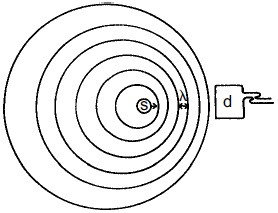
\includegraphics{Fig1_1a.jpg}}
\subfigure[Source moving from stationary detector d]{\label{fig:b}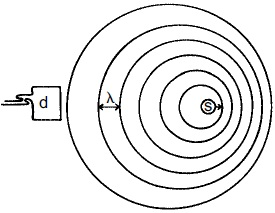
\includegraphics{Fig1_1b.jpg}}
\caption{Principles of Doppler Ultrasound}
\end{figure}
\noindent This is how you write equations and mathematical symbols:\\
\noindent In the Fig.1.1(a), an ultrasound source is moving with velocity $v_s$ toward the detector. After time $t$ following the production of any particular wave front, the distance between the wave front and the source is $(c$ - $v_s ) t$ , where $c$ is the velocity of ultrasound in the medium. The wavelength $\lambda$ of the ultrasound in the direction of motion is shortened to
\begin{equation}
\lambda = \frac{(c - v_s )}{\nu_0}
\end{equation}
\subsubsection{This  is a subsubsection} \label{This  is a subsubsection}
\noindent This is how you enter a single figure.Entering the caption automatically gives the figure its number, and the caption appears in the list of figures
\begin{figure}[H]
{\centering \resizebox*{4.8in}{2.8in}{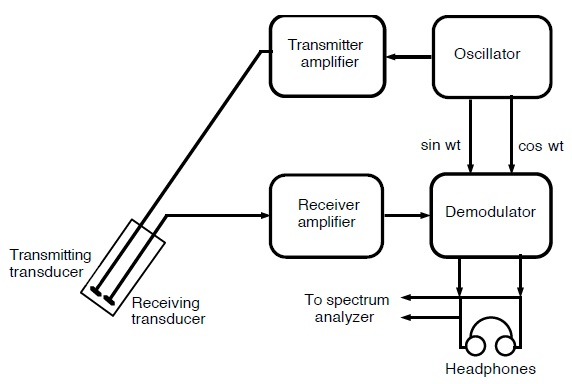
\includegraphics{Fig1_3.jpg}}\par}
\caption{The Continuous Wave Doppler system. Signals from the receiving transducers are compared in frequency to those transmitted.}
\end{figure}
\noindent This is an example of a table. You need to write the caption so that it appears here with its table no. as well as in the List of Tables.
\begin{table}[!ht]
\centering
\begin{tabular}{||c|c||}
\hline\hline
column1 & column2\\
\hline\hline
1st row 1st column & 1st row second column\\
\hline
2nd row 1st column & 2nd row 2nd column\\
\hline\hline
  \end{tabular}
  \caption{A test table.}
\end{table}
\pagebreak